\begin{figure}
	\centering
	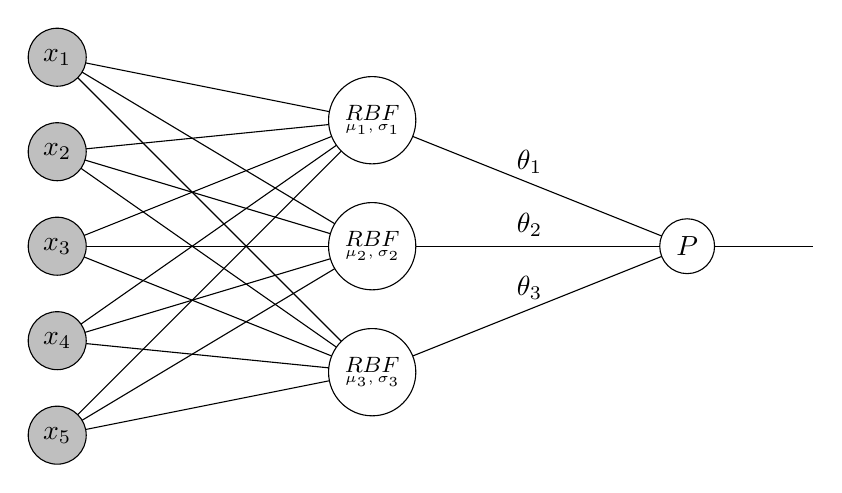
\begin{tikzpicture}[
		scale=0.8
	]

		\foreach \y in {-3,-1.5,0,1.5,3}{
			\foreach \yy in {-2,0,2}{
				\draw (-5,\y) -- (0,\yy);
			}
		}
	
		% input layer
		\foreach \y/\i in {3/1,1.5/2,0/3,-1.5/4,-3/5}{
			\node[circle,draw=black,fill=lightgray] at (-5,\y) {$x_{\i}$};
		}
		
		% rbf layer
		\foreach \y/\i in {-2/3,0/2,2/1}{
			\draw (0,\y) -- node[above] {$\theta_{\i}$} (5,0);
			\node[circle,draw=black,fill=white,align=center] at (0,\y)
				{\footnotesize $RBF$ \\[-3mm] \tiny $\mu_{\i}, \sigma_{\i}$};
		}

		% output layer
		\draw (5,0) -- ++(2,0);
		\node[circle,draw=black,fill=white] at (5,0) {$P$};
		
	\end{tikzpicture}
\end{figure}